%%%%%%%%%%%%
%
% $Autor: Wings $
% $Datum: 2019-03-05 08:03:15Z $
% $Pfad: SDCard $
% $Version: 4250 $
% !TeX spellcheck = en_GB/de_DE
% !TeX encoding = utf8
% !TeX root = filename 
% !TeX TXS-program:bibliography = txs:///biber
%
%%%%%%%%%%%%

\chapter{Arduino - SD-Karten-Modul}

Ein \ac{spi}-Lesegerät ist eine Art Modul, das die Kommunikation zwischen einem Mikrocontroller und einer Speicherkarte, z. B. einer \ac{sd}- oder \ac{tf}-Karte, ermöglicht. Das Modul verwendet das \ac{spi}-Protokoll, um Daten zwischen den beiden Geräten zu übertragen. Das \ac{sd}/\ac{tf}-Card-Shield-Modul ist ein spezieller Typ von \ac{spi}-Leser, der für die Verwendung mit Mikrocontroller-Boards konzipiert ist. Es ermöglicht einen einfachen Zugriff auf die auf der Speicherkarte gespeicherten Daten und kann für eine Vielzahl von Anwendungen wie Datenprotokollierung, Dateispeicherung und Multimedia-Projekte verwendet werden. Das Shield wird über die \ac{spi}-Schnittstelle mit dem Mikrocontroller verbunden.

\begin{figure}[h]
    \begin{center}
        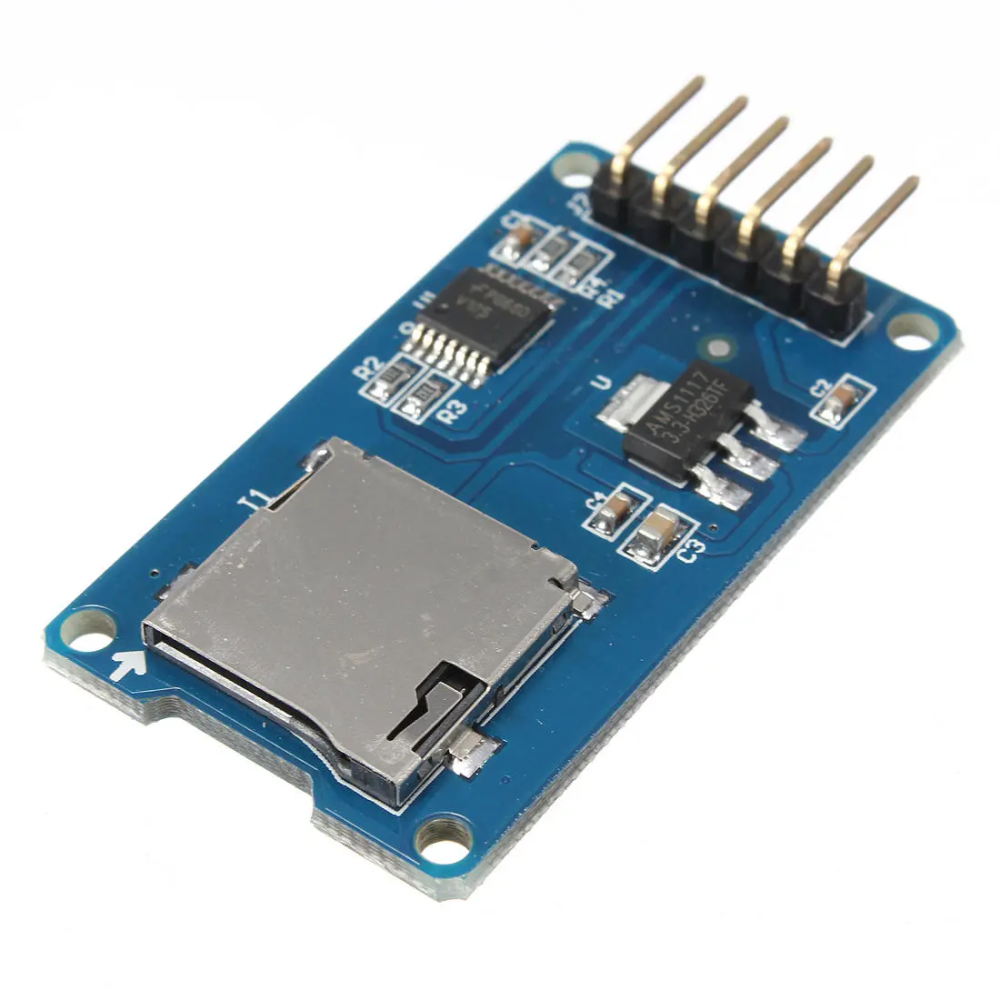
\includegraphics[width=12cm]{SDCard/SDCardSlot.png}
        \caption{SD/TF-Card-Shield-Modul}
        \label{fig:SD_Slot}
    \end{center}
\end{figure}

\section{Eigenschaften}

\begin{description}
    \item[Leichte und kostengünstige Erweiterung:] Der \ac{sd}-Karten Slot ermöglicht eine einfache und kostengünstige Erweiterung des Speicherplatzes für Ihr Arduino-Projekt mittels \ac{sd}-Karte.
    \item[Einfache Kommunikation:] Das Modul kommuniziert mit dem Mikrocontroller über das \ac{spi}-Protokoll, welches eine zuverlässige und schnelle Datenübertragung gewährleistet.
    \item[Unterstützung von Speicherkarten:] Es unterstützt sowohl Micro-SD-Karten (bis zu 2GB) als auch Micro-SDHC-Karten (bis zu 32GB), inklusive High-Speed-Karten.
    \item[Spannungsunterstützung:] Das Modul ist kompatibel mit einer Versorgungsspannung von 3,3-5V, was die Integration in verschiedene Projekte erleichtert.
\end{description}

\section{Technische Spezifikationen}

\begin{description}
    \item[Schnittstelle:] \ac{spi}
    \item[Unterstützte Karten:] Micro-SD-Karte (2GB), Micro-SDHC-Karte (bis zu 32GB)
    \item[Versorgungsspannung:] 3,3-5V
    \item[Kompatibilität:] Arduino und andere Mikrocontroller-Boards
\end{description}
\cite{AZ-Delivery:2021}



\section{Bibliothek \FILE{SD.h}}

Die SD.h Bibliothek ist eine essenzielle Bibliothek für Arduino-Entwickler, die es ermöglicht, \ac{sd}-Karten in ihren Projekten zu verwenden. Sie bietet eine einfache und effiziente Möglichkeit, Daten auf \ac{sd}-Karten zu speichern und zu lesen. Die Bibliothek unterstützt das FAT16 und FAT32 Dateisystem, was sie kompatibel mit den meisten \ac{sd}-Karten macht. Mit der SD.h Bibliothek können Dateien erstellt, gelöscht, umbenannt und bearbeitet werden. Zudem gibt es Funktionen zum Lesen und Schreiben von Daten in Dateien. Die Bibliothek ermöglicht das Erstellen und Löschen von Verzeichnissen (Ordnern) und unterstützt das Navigieren durch Verzeichnisse, was das Arbeiten mit komplexen Dateistrukturen erleichtert.

Die SD.h Bibliothek ist kompatibel mit den meisten Arduino-Boards, einschließlich Arduino Uno, Mega, Nano und anderen. Sie unterstützt sowohl Standard-\ac{sd}-Karten als auch microSD-Karten mit einem geeigneten Adapter. Die Integration der Bibliothek in Arduino-Sketches ist einfach und erfolgt durch leicht verständliche Methodenaufrufe. Die Arduino \ac{ide} enthält zudem Beispiele und umfangreiche Dokumentation, die den Einstieg in die Nutzung der SD.h Bibliothek erleichtern.


\section{Testen des SD-Karten Moduls}

Um das \ac{sd}-Karten Modul zu testen, haben wir ein Beispiel erstellt, das zeigt, wie man mit einem Arduino Daten auf einer \ac{sd}-Karte speichert und wieder ausliest. Basierend auf der Anleitung Funduino - Das \ac{sd}-Karten Modul haben wir den dortigen Beispielcode leicht angepasst \cite{AZ-Delivery:2021}. Zunächst wird die \ac{sd}-Karte initialisiert, um sicherzustellen, dass sie ordnungsgemäß funktioniert. Danach wird eine Testdatei erstellt, in die ein kurzer Text geschrieben wird. Anschließend wird der Inhalt dieser Datei ausgelesen und über den seriellen Monitor angezeigt.

\begin{code}[h]
    \pythonexternal[language=python]{../../Code/Arduino/SDCard/TestSDCard.ino}
    \caption{Testprogramm SD-Karten-Modul} 
    \label{Code:Test_SD_Karten_Modul}
\end{code}

\begin{figure}[h]
    \centering
    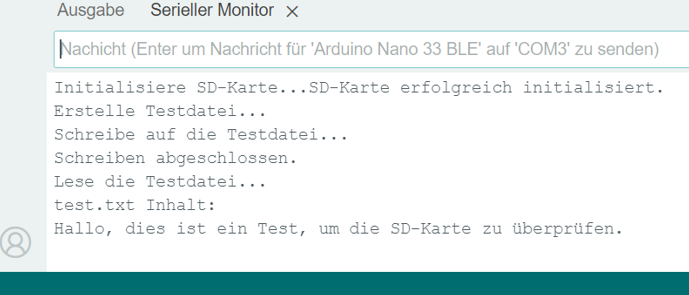
\includegraphics[width=10cm]{SDCard/SDCardTest}
    \caption{Ausgabe SD-Kartentest Serieller Monitor}
    \label{fig:SD_Kartentest_Serieller_Monitor}	
\end{figure}
